\section{Optimism in the Face of Uncertainty}
% Slide 14
\begin{frame}{Optimism in the Face of Uncertainty}
\centering
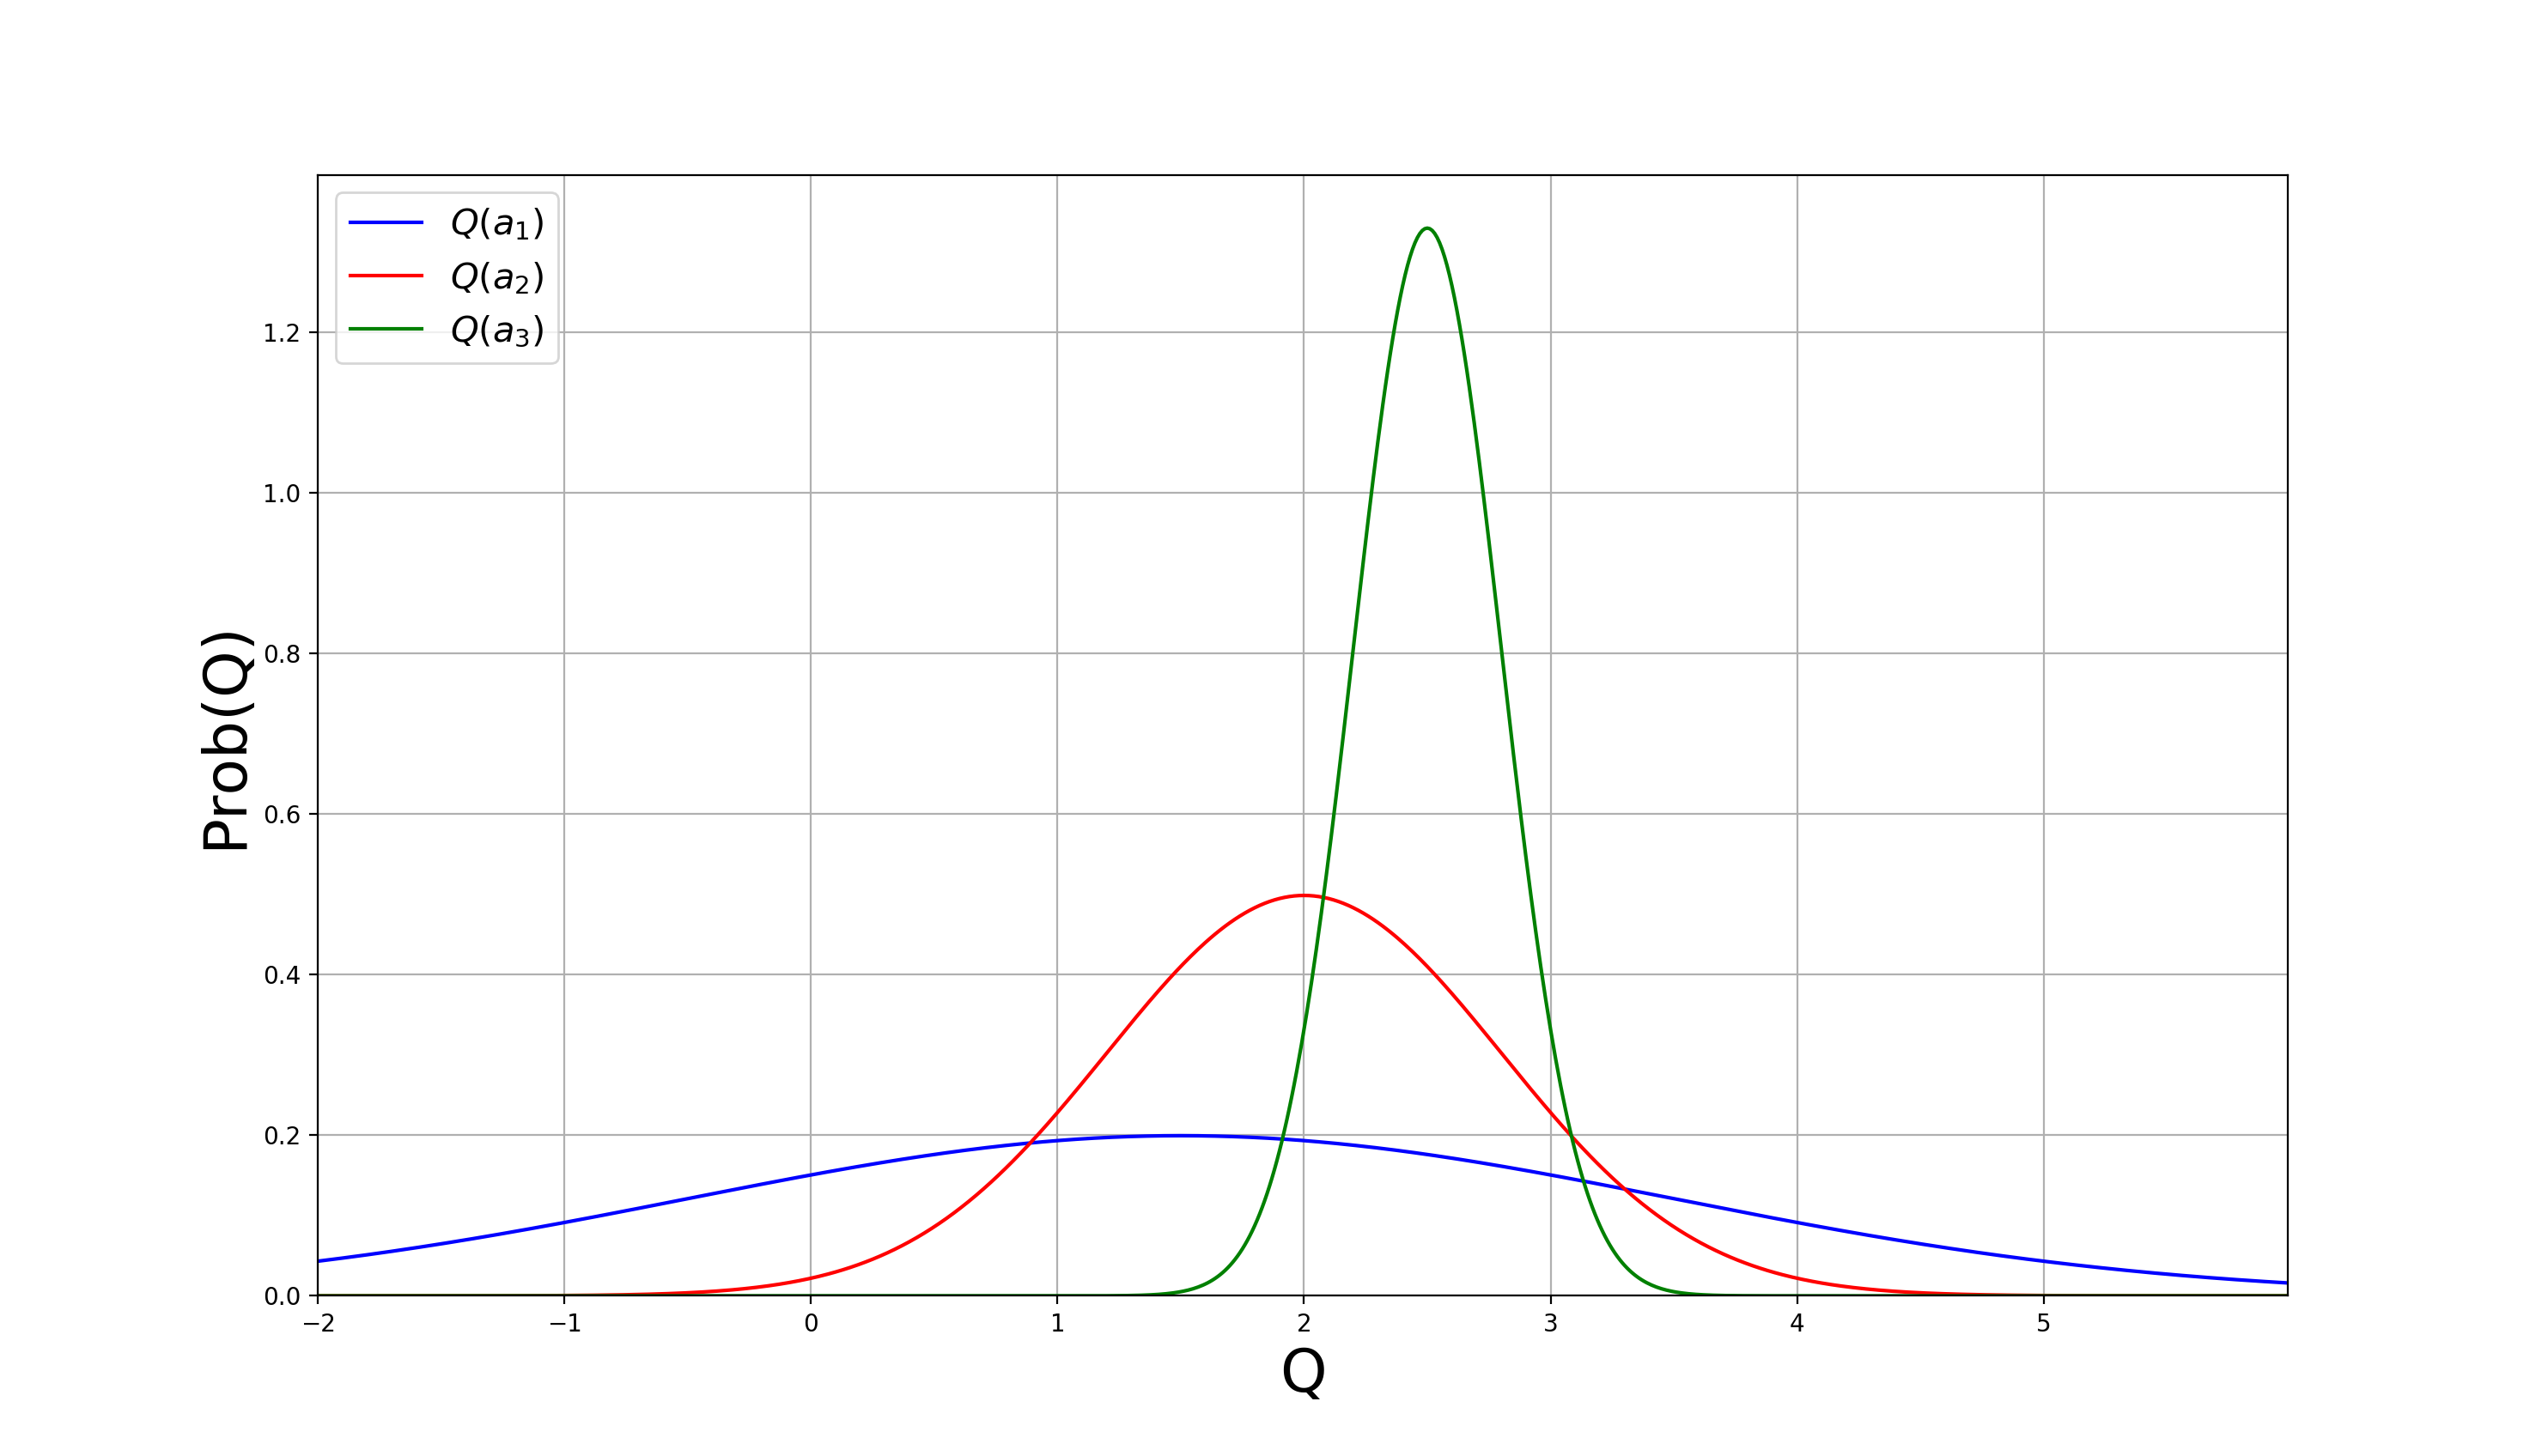
\includegraphics[width=0.62\textwidth,height=0.52\textheight,keepaspectratio]{images/bandits/figures/uncertainty-1.jpg}
\begin{itemize}
    \item Which action should we pick?
    \item The more uncertain we are about an action-value, the more
          important it is to explore that action
    \item It could turn out to be the best action
\end{itemize}
\end{frame}

% Slide 15
\begin{frame}{Optimism in the Face of Uncertainty (continued)}
\centering
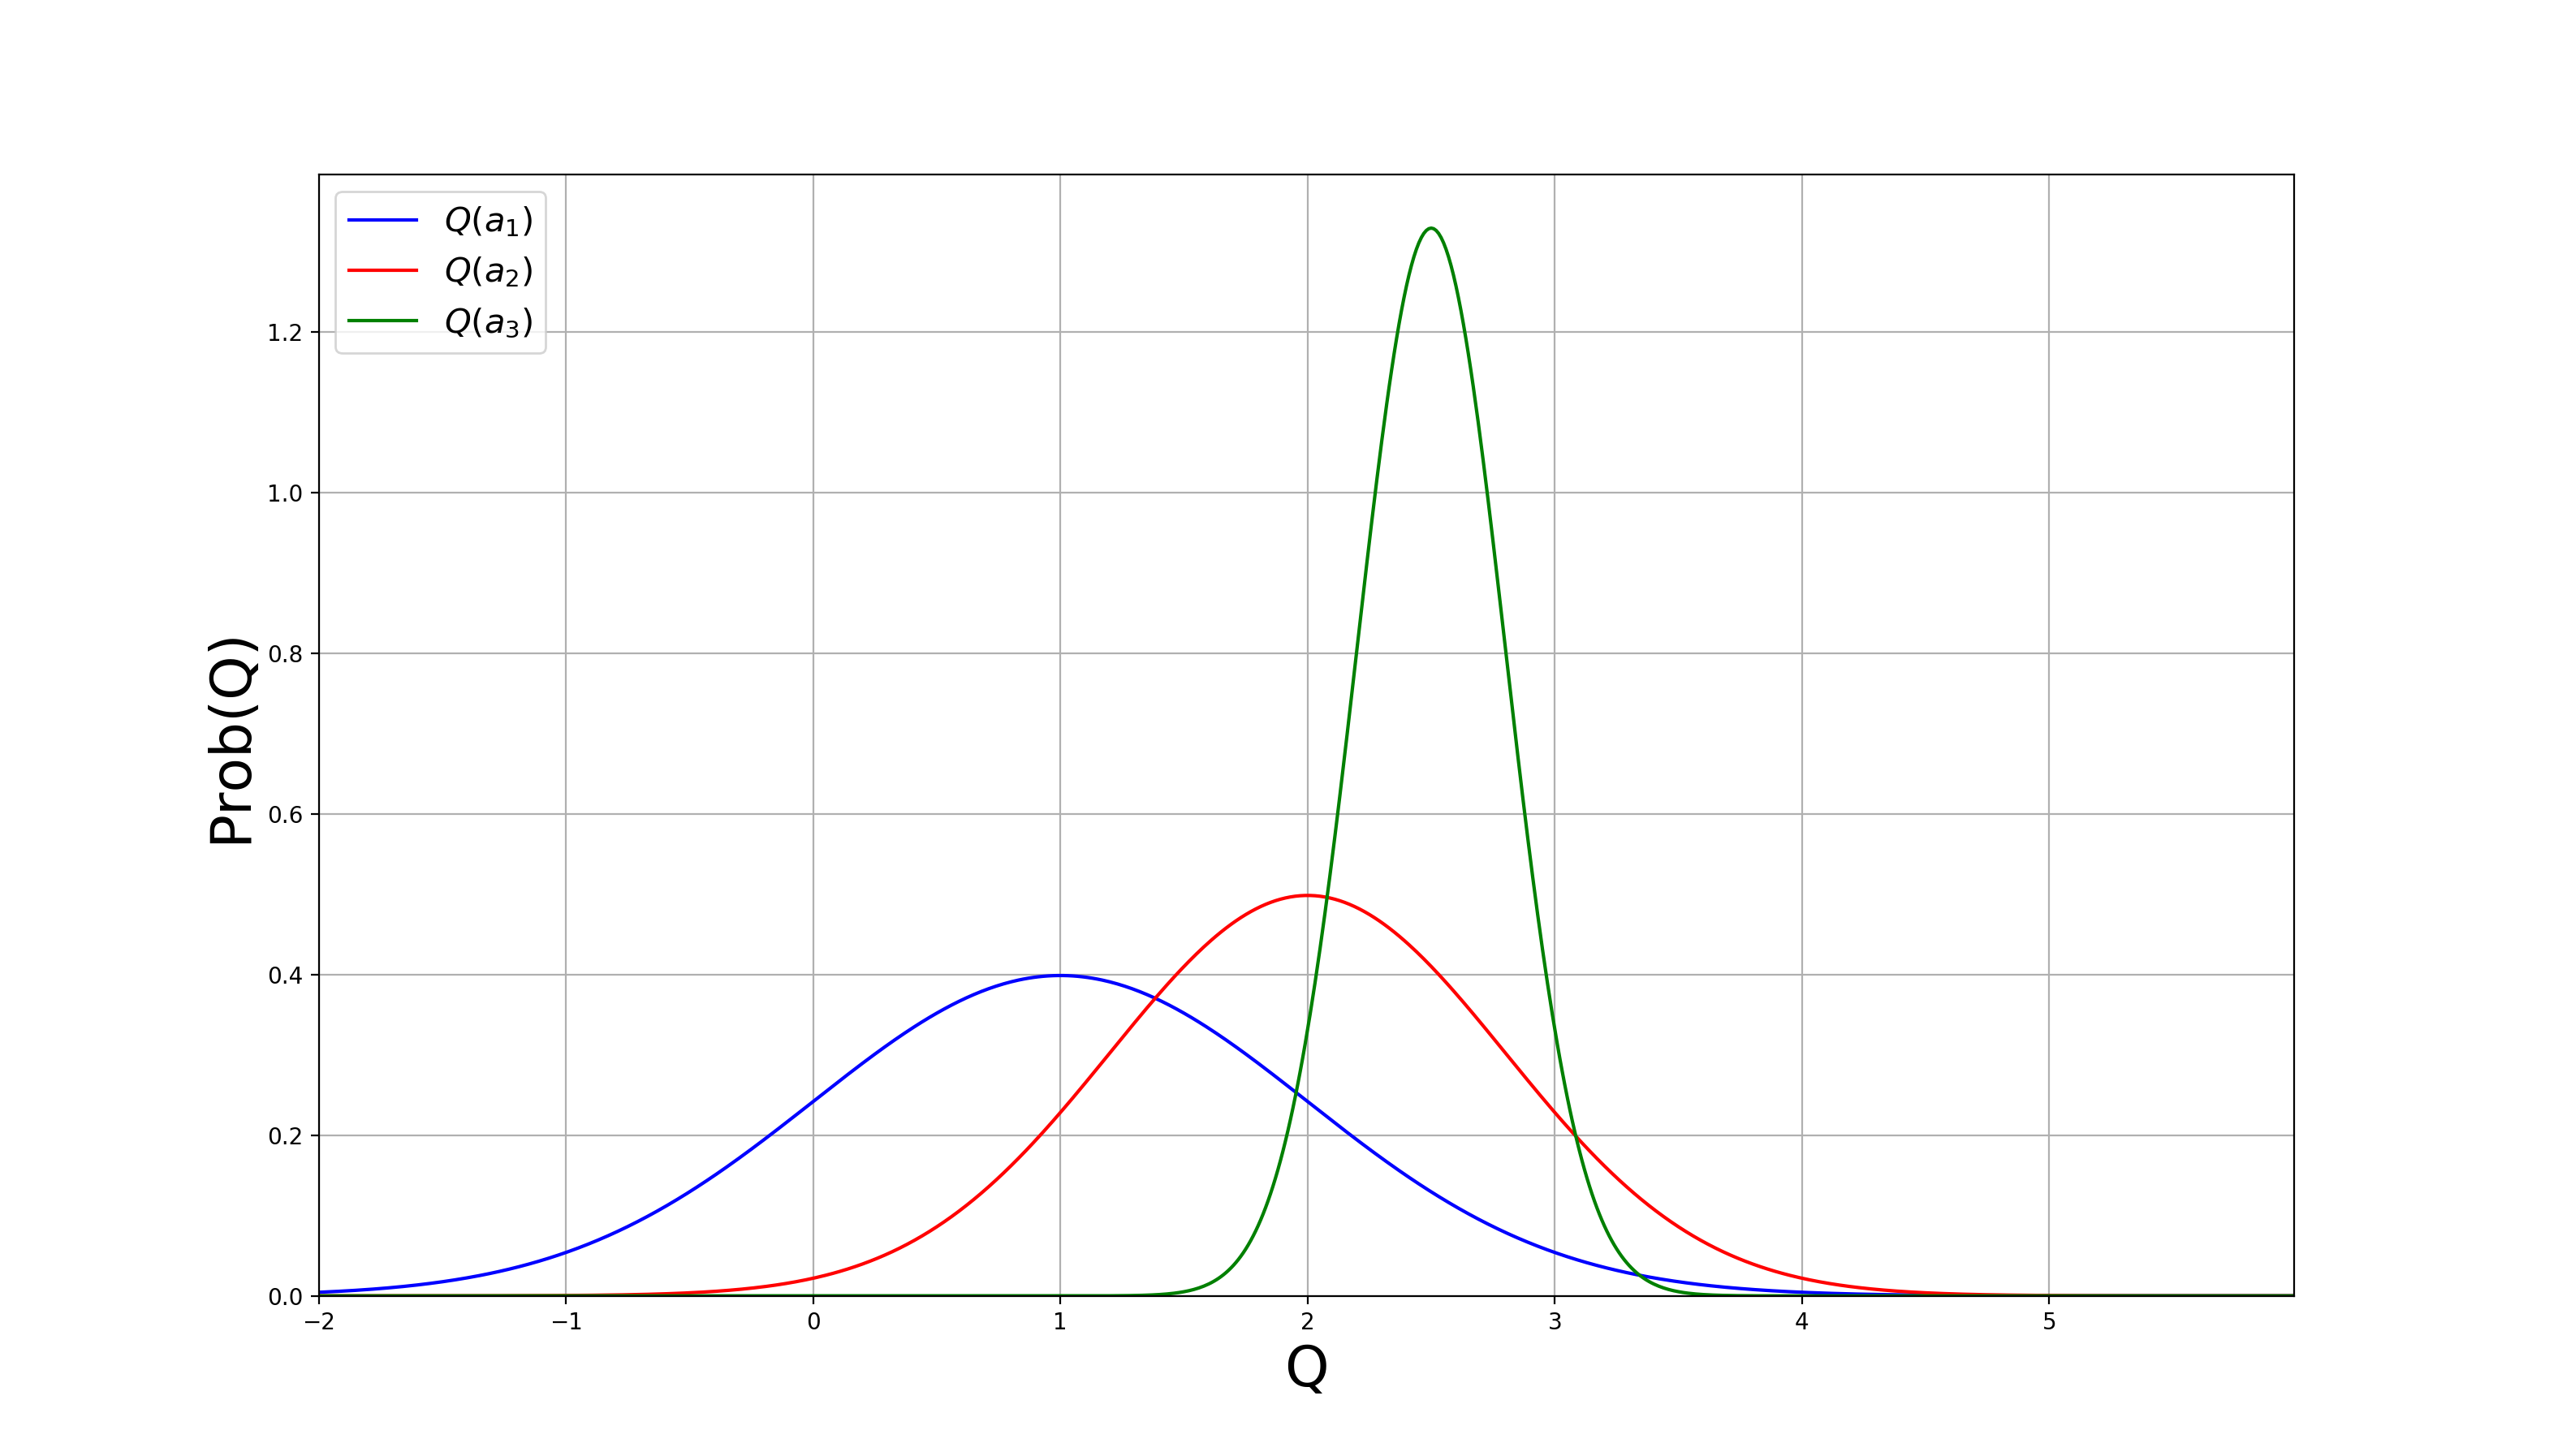
\includegraphics[width=0.62\textwidth,height=0.52\textheight,keepaspectratio]{images/bandits/figures/uncertainty-2.jpg}
\begin{itemize}
    \item After picking \emph{blue} action, we are less uncertain about the value
    \item And more likely to pick another action
    \item Until we home in on the best action
\end{itemize}
\end{frame}

% Slide 16
\begin{frame}{Upper Confidence Bounds}
\begin{itemize}
    \item Estimate an upper confidence $\hat{U}_t(a)$ for each action value
    \item Such that $Q(a) \leq \hat{Q}_t(a) + \hat{U}_t(a)$ with high probability
    \item This depends on the number of times $N_t(a)$ that $a$ has been selected
    \begin{itemize}
        \item Small $N_t(a) \Rightarrow$ Large $\hat{U}_t(a)$ (estimated value is uncertain)
        \item Large $N_t(a) \Rightarrow$ Small $\hat{U}_t(a)$ (estimated value is accurate)
    \end{itemize}
    \item Select action maximizing Upper Confidence Bound (UCB)
    \[
        a_{t+1} = \operatorname*{arg\,max}_{a \in \mathcal{A}} \left\{ \hat{Q}_t(a) + \hat{U}_t(a) \right\}
    \]
\end{itemize}
\end{frame}

% Slide 17
\begin{frame}{Hoeffding's Inequality}
\begin{block}{Theorem (Hoeffding's Inequality)}
Let $X_1, \ldots, X_n$ be i.i.d.\ random variables in $[0, 1]$, and let
\[
    \bar{X}_n = \frac{1}{n} \sum_{i=1}^{n} X_i
\]
be the sample mean. Then for any $u \geq 0$,
\[
    \mathbb{P}\!\left[\mathbb{E}[\bar{X}_n] > \bar{X}_n + u\right] \leq e^{-2nu^2}
\]
\end{block}
\begin{itemize}
    \item Apply Hoeffding's Inequality to rewards of $[0, 1]$-support bandits
    \item Conditioned on selecting action $a$ at time step $t$, setting $n = N_t(a)$
          and $u = \hat{U}_t(a)$,
    \[
        \mathbb{P}\!\left[Q(a) > \hat{Q}_t(a) + \hat{U}_t(a)\right] \leq e^{-2 N_t(a) \cdot \hat{U}_t(a)^2}
    \]
\end{itemize}
\end{frame}

% Slide 18
\begin{frame}{Calculating Upper Confidence Bounds}
\begin{itemize}
    \item Pick a small probability $p$ that $Q(a)$ exceeds UCB $\{\hat{Q}_t(a) + \hat{U}_t(a)\}$
    \item Now solve for $\hat{U}_t(a)$
    \begin{align*}
        e^{-2 N_t(a) \cdot \hat{U}_t(a)^2} &= p \\
        \Rightarrow \hat{U}_t(a) &= \sqrt{\frac{-\log p}{2 N_t(a)}}
    \end{align*}
    \item Reduce $p$ as we observe more rewards, eg: $p = t^{-\alpha}$ (for fixed $\alpha > 0$)
    \item This ensures we select optimal action as $t \to \infty$
    \[
        \hat{U}_t(a) = \sqrt{\frac{\alpha \log t}{2 N_t(a)}}
    \]
\end{itemize}
\end{frame}

% Slide 19
\begin{frame}{UCB1}
Yields UCB1 algorithm for arbitrary-distribution arms bounded in
$[0, 1]$
\[
    a_{t+1} = \operatorname*{arg\,max}_{a \in \mathcal{A}} \left\{ \hat{Q}_t(a) + \sqrt{\frac{\alpha \log t}{2 N_t(a)}} \right\}
\]
\begin{block}{Theorem}
The UCB1 Algorithm achieves logarithmic total regret
\[
    L_T \leq \sum_{a \mid \Delta_a > 0} \frac{4\alpha \cdot \log T}{\Delta_a} + \frac{2\alpha \cdot \Delta_a}{\alpha - 1}
\]
\end{block}
\href{https://github.com/TikhonJelvis/RL-book/tree/master/rl/chapter14/ucb1.py}{Educational Code} for UCB1 algorithm
\end{frame}
